\section{Die Benutzerschnittstelle}
	In diesem Abschnitt dieses Kapitels wird auf die Implementierung der Benutzerschnittstelle eingegangen. Wie schon bereits im SRS erwähnt handelt es sich bei der Benutzerschnittstelle um die grafische Oberfläche der Android App. Dafür wird zunächst auf die Umsetzung eingegangen und abschließend die Auswertung der Benutzeroberfläche mit einem Usability Test behandelt.
		
	\subsection{Die Umsetzung}	
		Um die ergonomie zu erhöhen kann der linke joystick i einem festgelegten bereich überall angelegt werden
		
		Da es sich um KOmponenten handelt die immer da sein müssen wurde sich für das normale UI Screen Space - OVerlay ausgewählt
		
		\begin{figure}[htbp]
			\centering 
			\label{alwaysOnUI}
			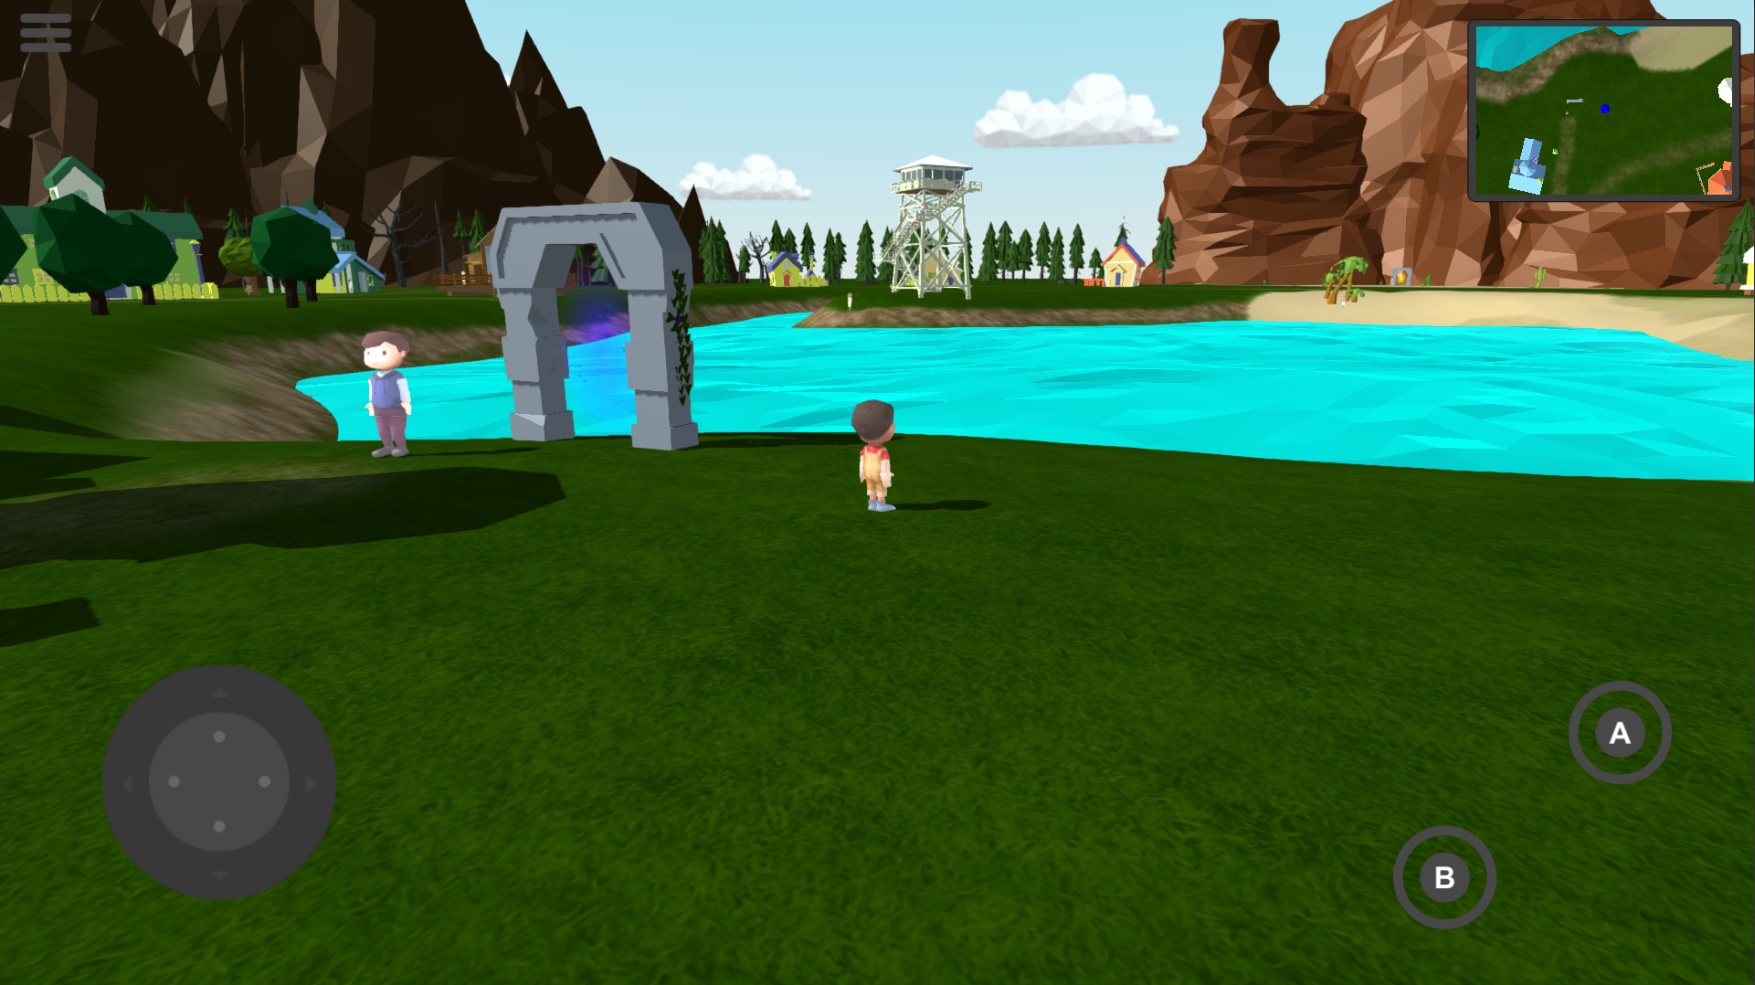
\includegraphics[width=13cm]{pics/alwaysOnUI.png}
			\caption{User Interface: Head-Up Display}
		\end{figure}
	
		\begin{figure}[htbp]
			\centering 
			\label{userInterfaces}
			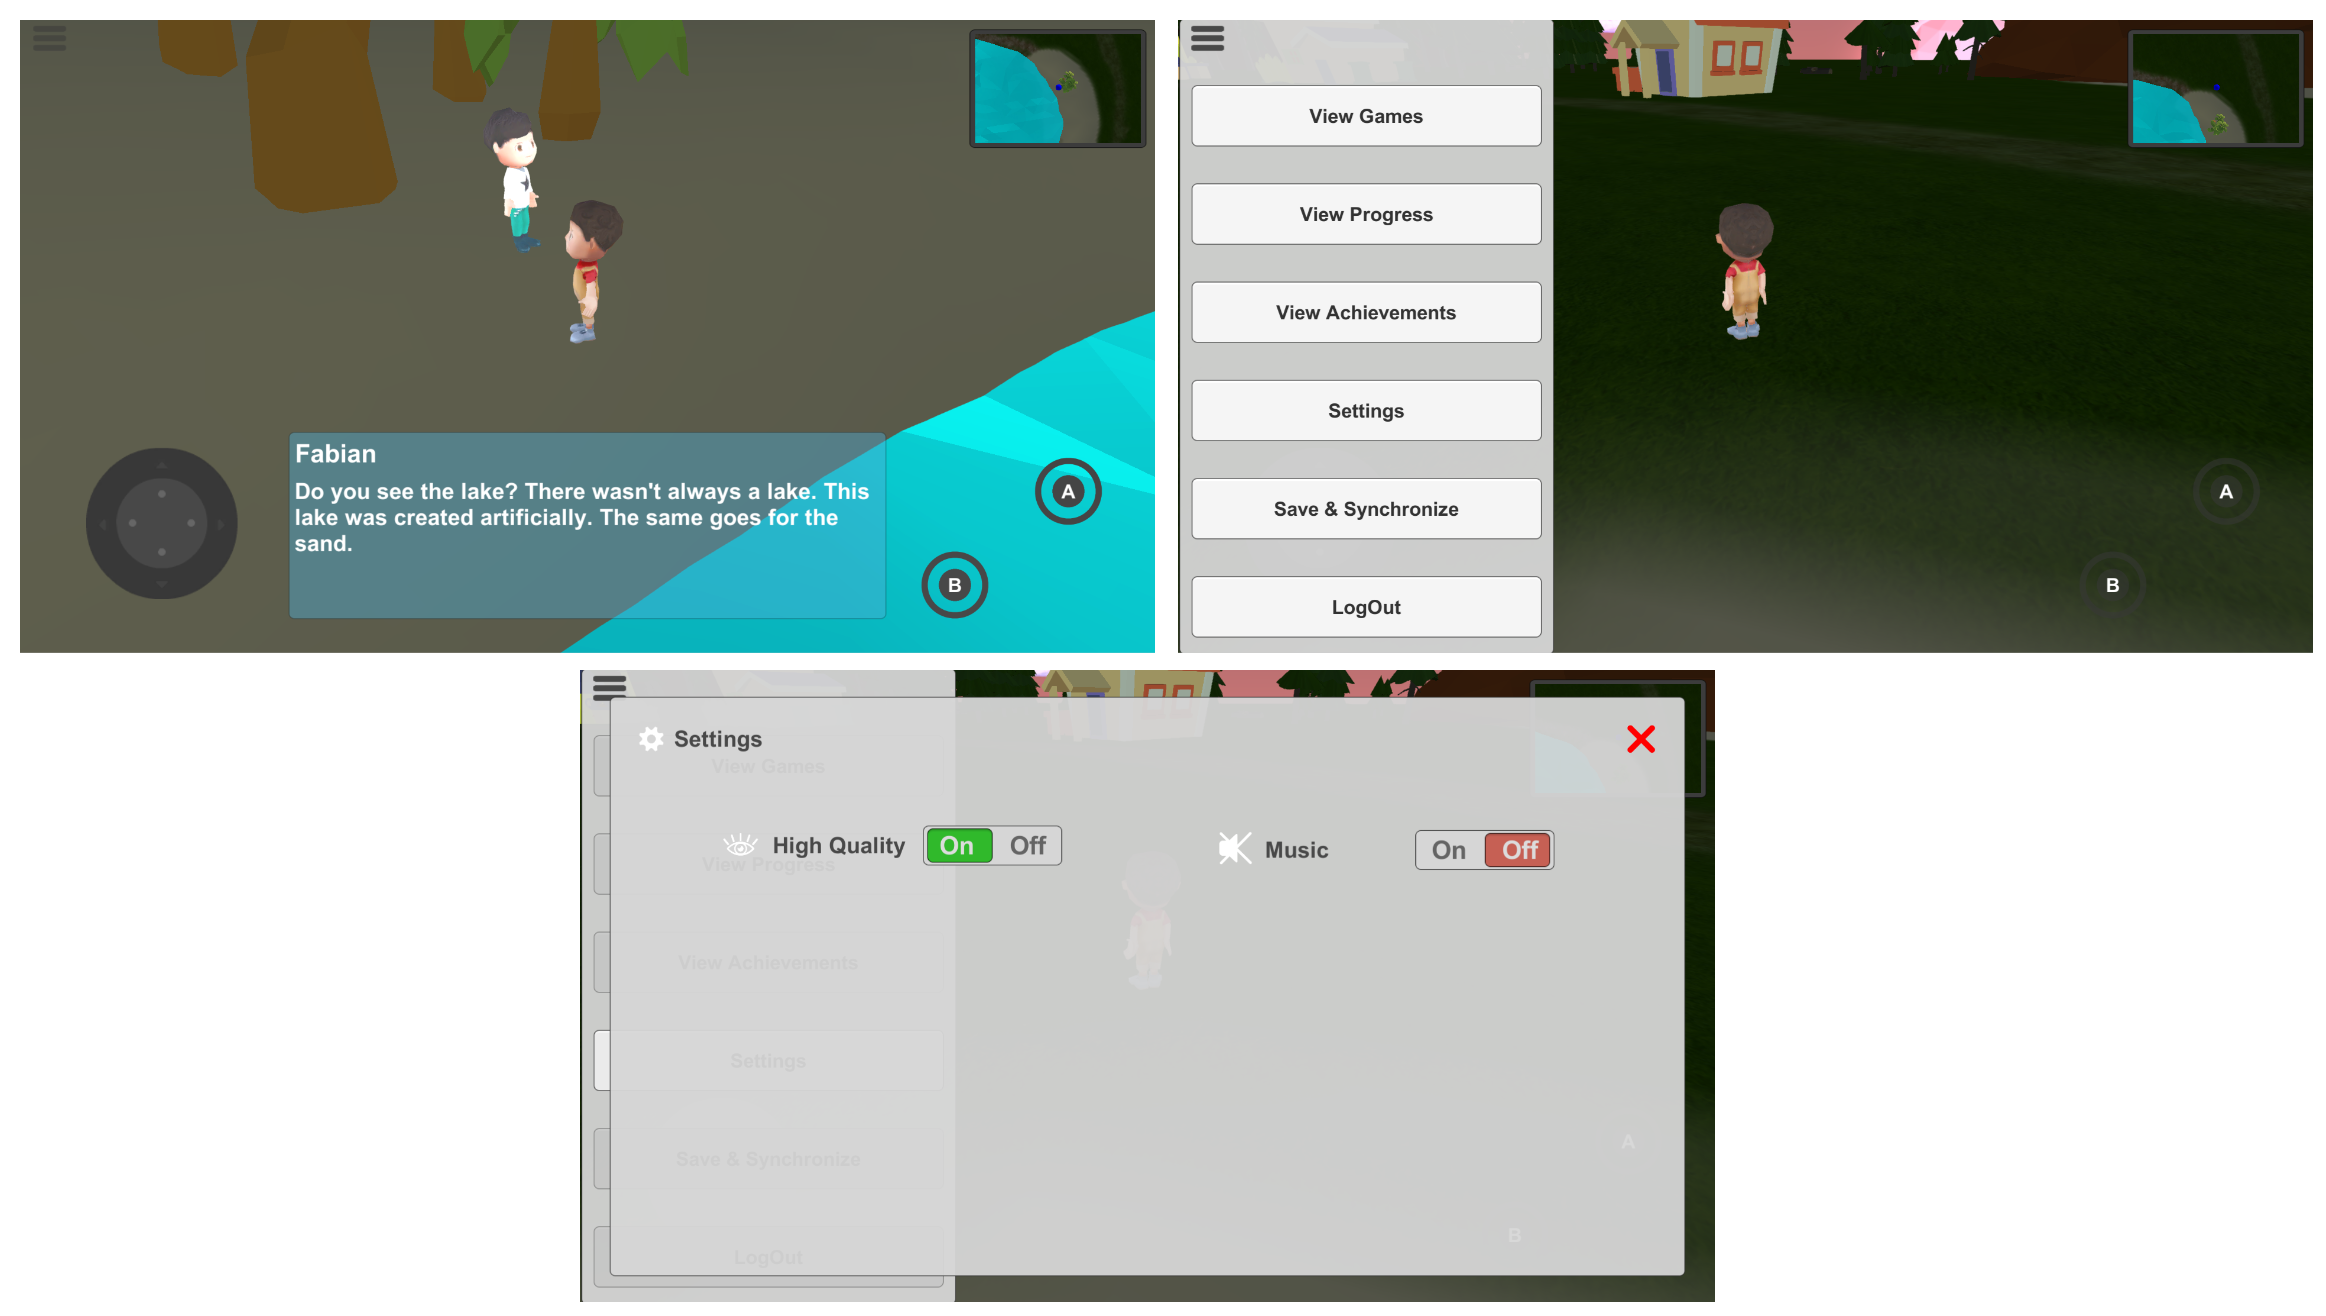
\includegraphics[width=\textwidth]{pics/userInterface.png}
			\caption{User Interfaces: Kommunikation, Menu und Einstellungen-Fenster}
		\end{figure}
	
		Menu fenster bildet die erste Dialogebene nach der Startebene. Nach diesem gibt es noch eine weitere Ebene. dieser Dialog dient zum Abbrechen, warnt vor bevorstehenden Aktionen. Die maximale Dialogebene ist also 2. 

		\begin{figure}[htbp]
			\centering 
			\label{RegisterUI}
			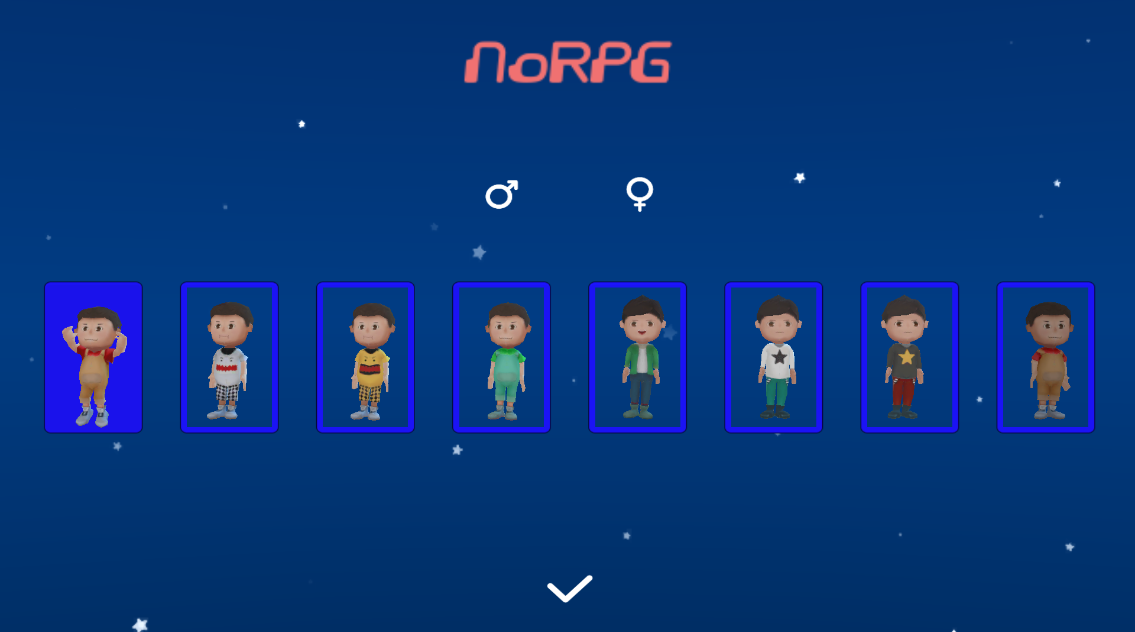
\includegraphics[width=13cm]{pics/RegisterUI.png}
			\caption{User Interface: Registrierung}
		\end{figure}

	
	\subsection{Usability Evaluation}
		Ein Usability Test wird durchgeführt, um die Gebrauchstauglichkeit einer Software oder Hardware mit den potenziellen Benutzern zu überprüfen. Usability wird durch die Attribute Erlernbarkeit, Effizienz, Einprägsamkeit, Fehlerrate und Zufriedenheit\footnote{Vgl. Nielsen \cite{NielsenUI} Seite 26} beschrieben. Unter dem Attribut Erlernbarkeit beschreibt Nielsen in seinem Buch, dass die Anwendung leicht zu erlernen sein muss, damit der Benutzer in kurzer Zeit beginnen kann das Spiel zu spielen. Dazu zählt beispielsweise die Steuerung. Diese ist wichtig, damit der Benutzer sich im Spiel intuitiv bewegen kann. So bald der Spieler das System gelernt und verstanden hat, soll ein hohes Maß an Produktivität möglich sein. Dies wird als Effizienz bezeichnet. Das System sollte allerdings leicht zu merken und einprägsam sein, so dass auch der Gelegenheitsbenutzer in der Lage ist, nach einer gewissen Zeit ohne Verwendung der Anwendung, in das Spiel zurückzukehren, ohne alles nochmals neu lernen zu müssen. Nielsen weißt zudem darauf hin, dass Fehler für den Benutzer sehr frustrierend sein können. Daher sollte das System eine geringe Fehlerquote haben, so dass Benutzer bei der Verwendung nur wenig Fehler machen und falls Probleme auftauchen, diese den Spaß am Spielen nicht einschränken. Das letzte Attribut beschreibt den Gesamteindruck\footnote{Vgl. Nielsen \cite{NielsenUI} Seite 27ff.}.
		
		Es wird zwischen formativem und summativem Usability Test unterschieden. Foramtive Tests werden während der Entwicklung durchgeführt. Die Aufgabe ist es ein spezielles Problem bzw. Szenario zu testen. Es handelt sich dabei um eine kleine Studie für schnelles Feedback, welche wiederholt durchgeführt werden kann\footnote{Vgl. Rubin und Chisnell \cite{handbookUsability} Seite 29f.}. Der summative Test findet einmalig nach der Entwicklung statt, bevor das fertige Produkt ausgeliefert wird. Dabei handelt es sich um eine umfangreiche Studie, die alle Funktionen der Benutzeroberfläche bewertet\footnote{Vgl. Rubin und Chisnell \cite{handbookUsability} Seite 34f.}.
		
		Ein Usabilty Test kann in verschiedenen Testumgebungen durchgeführt werden. Es wird zwischen Labortest, Feldtest und Remotetest unterschieden. Bei einem Labortest handelt es sich entweder um ein Usability Labor oder um einen allgemein nutzbaren Raum. Der ausschlaggebende Unterschied zwischen diesen beiden ist, dass das Usability Labor nur für Usabilty Tests und Evaluationen verwendet wird. Die potenziellen Tester werden eingeladen und führen die Auswertung in diesem Raum durch. Zu den Basisutensilien gehört neben Nahrung und Verpflegung die notwendige Hardware und Software, sowie ein Moderator bzw. Experte für Fragen und Probleme\footnote{Vgl. Rubin und Chisnell \cite{handbookUsability} Seite 101f.}. Der Feldtest oder auch Mobiler Test kann potentiell überall durchgeführt werden, sei es beim Kunden, in einem öffentlichen Gebäude oder in einem Café. Der Vorteil im Vergleich zu einem Labortest ist, dass der Benutzer sich einer gewohnten und reale Umgebung mit echten Lichtverhältnissen befindet. Allerdings ist es wahrscheinlicher das der Tester durch die Umwelt abgelenkt wird\footnote{Vgl. Rubin und Chisnell \cite{handbookUsability} Seite 98f.} und der Experte mit zum Kunden. Bei der letzten Möglichkeit ist der Benutzer und Moderator örtlich voneinander getrennt. Der Remotetest kann synchron, indem der Moderator und die Teilnehmer per Audio- oder Videokonferenz verbunden sind, oder asynchron stattfinden. Der wesentliche Vorteil ist, dass dadurch potenziell mehr Testpersonen teilnehmen und es günstiger ist. Allerdings können keine komplexen Anforderungen gestellt werden und bei Fragen ist der Tester mehr oder weniger auf sich gestellt.
		
		Bei der in diesem Kapitel beschrieben Evaluation handelt es sich um einen summativen Remotetest. Der Usability Test findet erst nach der Entwicklung von NoRPG statt und nachdem alle Funktionen implementiert wurden. Die Gründe für einen Remotetest sind, da eine es sich bei NoRPG um eine mobile Anwendung handelt und diese am besten auf dem eigenen Smartphone getestet werden kann. Dadurch werden auch verschiedenste Hardware und Android Versionen geprüft und validiert. Ein weiterer essentieller Punkt sind die Kosten. In dem Umfang dieser Studienarbeit ist es nicht möglich ein Feldtest oder Labortest durchzuführen.
	
		In der Vorbereitung des Usability Tests gilt es zunächst die Benutzerprofile zu erstellen, die zu testenden Szenarien und Ziele, sowie den Umfang zu definieren. Anschließend die Unterlagen vorzubereiten, die Teilnehmer zu rekrutieren und den Zeitraum festzulegen. Das Profil für die Tester ist das gleiche wie das der potenziellen Spieler. Daher wird kein festes Profil für die Evaluation festgelegt, da NoRPG für jung oder alt und männlich oder weiblich ausgelegt ist. Jedoch gilt bei der Rekrutierung zu beachten, das von jeder Alters- und Geschlechtsgruppe eine gewisse Anzahl vertreten ist.
		
		Das Ziel dieser Evaluation ist das Testen der Benutzeroberfläche, da es sich bei einer mobilen Anwendung um die einzige Interaktionsschnittstelle für die Benutzer handelt. Aus diesem Grund ist eine fehlerfreie, intuitive und gleichzeitig gut aussehende Benutzeroberfläche sehr wichtig. Zu den abzubildenden Szenarios gehört zum Beispiel die Registrierung, der Log-In oder die Liste der heruntergeladenen Spiele. Alle User Interface Elemente sollen in diesem summativen Test geprüft und evaluiert werden.
		
		Umfang 
		
		Zeitraum 
		
		Für das Usability Test wurde ein Formular für die Tester erstellt. Dieses beinhaltet genau alle Information und Schritte die notwendig sind um die Funktionen, die verschiedene UI Elemente hervorbringen, zu testen und anschließend evaluieren zu können.
